\documentclass[12pt, a4paper]{article}

% ─── Packages ───────────────────────────────────────────────────────────────
\usepackage[a4paper, margin=1in]{geometry}
\usepackage{times}
\usepackage{graphicx}
\usepackage{amsmath}
\usepackage{array}
\usepackage{booktabs}
\usepackage{hyperref}
\usepackage{caption}
\usepackage{subcaption}
\usepackage{listings}
\usepackage{xcolor}
\usepackage{titlesec}
\usepackage{enumitem}
\usepackage{cite}
\usepackage{fancyhdr}
\setlength{\headheight}{15pt}
\usepackage{setspace}
\usepackage{parskip}
\usepackage{microtype}
\usepackage{float}

% ─── Hyperref Setup ─────────────────────────────────────────────────────────
\hypersetup{
  colorlinks=true,
  linkcolor=black,
  citecolor=black,
  urlcolor=blue
}

% ─── Section Title Formatting ───────────────────────────────────────────────
\titleformat{\section}{\large\bfseries\uppercase}{{\thesection.}}{0.5em}{}
\titleformat{\subsection}{\normalsize\bfseries}{{\thesubsection}}{0.5em}{}
\titleformat{\subsubsection}{\normalsize\itshape}{{\thesubsubsection}}{0.5em}{}

% ─── Code Listing Style ──────────────────────────────────────────────────────
\lstdefinestyle{cppstyle}{
  language=C++,
  basicstyle=\footnotesize\ttfamily,
  keywordstyle=\color{blue}\bfseries,
  commentstyle=\color{gray}\itshape,
  stringstyle=\color{teal},
  numberstyle=\tiny\color{gray},
  numbers=left,
  stepnumber=1,
  numbersep=8pt,
  frame=single,
  breaklines=true,
  captionpos=b,
  tabsize=2,
  backgroundcolor=\color{gray!5}
}

% ─── Header / Footer ────────────────────────────────────────────────────────
\pagestyle{fancy}
\fancyhf{}
\lhead{\small Smart Medicine Cabinet Tracker}
\rhead{\small NIT Hamirpur, 2026}
\cfoot{\thepage}
\renewcommand{\headrulewidth}{0.4pt}

% ─── Document ───────────────────────────────────────────────────────────────
\begin{document}

\begin{titlepage}
    \centering
    \vspace*{0.5cm}

    {\Large \textbf{Smart Medicine Cabinet Tracker: IoT-Based RFID Medicine\\
    Management with Expiry Monitoring and Dose Scheduling}\par}

    \vspace{1.5cm}

    {\large Dual Degree, CS-744, Internet of Things, Project Report\par}

    \vspace{1.5cm}

    {\large Submitted By\par}
    \vspace{0.3cm}
    {\large \textbf{Anirudh Sharma (22dcs002)}\par}

    \vspace{1.5cm}

    {\large Under the Guidance of\par}
    \vspace{0.3cm}
    {\large \textbf{Dr. Robin Singh Bhadoria}\par}
    {\small Assistant Professor, Department of CSE\par}

    \vfill

    
\includegraphics[width=0.25\textwidth]{images/nith_logo.png}\par
    \vspace{0.5cm}

    {\normalsize \textbf{Department of Computer Science and Engineering}\par}
    \vspace{0.2cm}
    {\normalsize \textbf{NATIONAL INSTITUTE OF TECHNOLOGY HAMIRPUR}\par}
    \vspace{0.1cm}
    {\normalsize Hamirpur (Himachal Pradesh) -- 177005, India\par}
    \vspace{0.3cm}
    {\normalsize April 2026\par}

\end{titlepage}

% ─── Table of Contents ──────────────────────────────────────────────────────
\tableofcontents
\newpage

% ─── Abstract ───────────────────────────────────────────────────────────────
\begin{center}
    \Large\textbf{Abstract}
\end{center}
\vspace{0.5cm}

\noindent
Medication non-adherence and improper storage conditions are leading causes of treatment failure and medicine wastage worldwide. This paper presents the design, implementation, and simulation-based validation of a Smart Medicine Cabinet Tracker—an IoT-based embedded system built around the Arduino Uno R3 microcontroller. The system employs an MFRC522 RFID reader to uniquely identify individual medicine containers, a DS1307 Real-Time Clock module for time-stamped expiry computation and dose scheduling, and a DHT22 sensor for continuous cabinet temperature and humidity monitoring. Medicines are registered and managed via a 4$\times$4 matrix keypad with a 16$\times$2 I\textsuperscript{2}C LCD providing real-time feedback. A structured EEPROM storage scheme retains up to 21 medicine records—including name, quantity, expiry date, and dosage interval—across power cycles. An alert classification algorithm drives a three-colour LED array and piezo buzzer with distinct patterns for five hazard categories: medicine expiry, impending expiry, missed doses, temperature excursion, and high humidity. All five alert scenarios were successfully validated through simulation. The estimated unit hardware cost is approximately INR~950--1,200, making the system a practical and low-cost alternative to commercial smart pill dispensers.

\vspace{0.6cm}
\noindent\textbf{Keywords:} IoT, Arduino Uno R3, RFID, MFRC522, DS1307, EEPROM, Medicine Management, Dose Tracking, Expiry Monitoring, DHT22

\newpage

% ─── 1. Introduction ────────────────────────────────────────────────────────
\section{Introduction}

\subsection{Background and Motivation}

Medication non-adherence is a pervasive global health challenge. The World Health Organization (WHO) reports that approximately 50\% of patients with chronic illnesses fail to take their medications as prescribed, resulting in avoidable hospitalizations, disease progression, and an estimated economic burden exceeding USD~100~billion annually \cite{who_adherence}. Beyond adherence, improper storage of temperature-sensitive drugs—such as insulin, biologics, and certain antibiotics—leads to degraded efficacy or outright toxicity. Most households and small clinics lack any automated mechanism to track medicine expiry dates, monitor storage conditions, or alert caregivers to missed doses.

Embedded IoT systems combining RFID identification, real-time clocks, environmental sensing, and local actuation offer a practical and cost-effective pathway to address these gaps without requiring continuous internet connectivity. The Smart Medicine Cabinet Tracker presented in this work is designed to operate fully at the edge: all tracking logic, alert evaluation, EEPROM persistence, and display are handled by a low-cost Arduino Uno R3 node, with no network dependency.

\subsection{Literature Review}
\label{sec:related}

Several recent works have addressed IoT-based pharmaceutical monitoring and medication management, each exhibiting specific limitations that this work targets.

Jiang et al.\ \cite{jiang2024} proposed a sustainable IoT framework targeting energy optimization in edge monitoring nodes for pharmaceutical cold-chain applications. Their system achieved a 22\% reduction in energy consumption and 99.8\% thermal compliance in real-time tests. However, the approach incurs high initial setup costs and requires continuous network connectivity, making it unsuitable for household or low-resource clinical settings.

Sujiya et al.\ \cite{sujiya2025} developed a multi-sensor node architecture for continuous pharmaceutical transit monitoring with an alert latency under 2~seconds and 98\% fault detection accuracy. Their system monitors only temperature and humidity, omitting RFID-based medicine identification, dose scheduling, and expiry tracking—gaps directly addressed in this work.

Hasanat et al.\ \cite{hasanat2024} designed a smart active vaccine carrier integrating long-range communications for last-mile delivery, achieving 48-hour active uptime and 99\% communication success. The approach proposes complex carrier hardware but lacks medicine-level identification or dose management features.

Enriko et al.\ \cite{enriko2023} presented an end-to-end tracking and cloud logging framework for pharmaceutical distribution, demonstrating reliable visibility across a logistics chain. The system is heavily dependent on continuous network connectivity and provides no edge-based medicine cabinet management.

Ali and Khan \cite{ali2023} evaluated IoT platforms for pharmaceutical logistics using multi-criteria decision-making models. While the work provides useful platform guidance, it does not contribute a real embedded implementation or medicine-level tracking strategy.

\smallskip
\noindent\textbf{Gap Analysis:} No prior work combines (i) RFID-based per-medicine identification, (ii) RTC-driven expiry date computation and dose scheduling, (iii) multi-threshold environmental monitoring with alert classification, and (iv) complete offline EEPROM persistence—all within a single low-cost, simulation-validated Arduino prototype. This work bridges that gap.

\begin{table}[H]
\centering
\caption{Comparison of Related Works}
\label{tab:related}
\renewcommand{\arraystretch}{1.3}
\begin{tabular}{p{2.8cm} p{2.6cm} p{2.4cm} p{3.4cm}}
\toprule
\textbf{Reference} & \textbf{Sensors / ID} & \textbf{Offline / Alert} & \textbf{Key Limitation} \\
\midrule
Jiang et al., 2024 \cite{jiang2024}     & Temp, Energy       & No / Yes  & High cost; network-dependent \\
Sujiya et al., 2025 \cite{sujiya2025}   & Temp, Humidity     & Yes / Yes & No RFID; no dose tracking \\
Hasanat et al., 2024 \cite{hasanat2024} & GPS, Temp          & No / Yes  & No medicine-level ID \\
Enriko et al., 2023 \cite{enriko2023}   & Location, Temp     & No / Yes  & No edge management \\
\textbf{This Work}                      & RFID, Temp, Hum, RTC & Yes / Yes & Simulation only; no cloud \\
\bottomrule
\end{tabular}
\end{table}

\subsection{Objectives}

The objectives of this work are:
\begin{enumerate}[label=(\roman*)]
  \item Design an RFID-based IoT node capable of uniquely identifying individual medicine containers and maintaining per-medicine records in EEPROM.
  \item Implement an RTC-driven expiry date computation algorithm that raises timely alerts for medicines nearing or past their expiry date.
  \item Develop a dose tracking subsystem that monitors scheduled dosage intervals and generates escalating missed-dose alerts.
  \item Integrate environmental monitoring via DHT22 to enforce safe temperature and humidity storage conditions.
  \item Validate the complete system through simulation, demonstrating reliable detection of all five monitored hazard categories.
\end{enumerate}

\subsection{Scope and Organization}

This paper is organized as follows: Section~\ref{sec:problem} defines the problem; Section~\ref{sec:architecture} describes the system architecture and design; Section~\ref{sec:components} details the hardware components; Section~\ref{sec:implementation} covers the firmware implementation; Section~\ref{sec:results} presents simulation results and discussion; Section~\ref{sec:future} discusses future integration and large-scale applications; Section~\ref{sec:conclusion} concludes the work.

% ─── 2. Problem Statement ────────────────────────────────────────────────────
\section{Problem Statement}
\label{sec:problem}

Households, elderly care facilities, and small clinics routinely manage multiple medicines simultaneously. The current state of practice suffers from three interconnected problems.

\textbf{1. Manual and error-prone expiry management.} Medicine expiry dates are printed on labels that users must visually inspect—a task easily neglected, especially for medicines stored in opaque containers or stacked behind others. Expired medicines, if inadvertently administered, can cause treatment failure or adverse reactions.

\textbf{2. Missed or duplicate dosing.} Patients—particularly the elderly managing several medications—frequently miss doses or accidentally take double doses in the absence of an automated tracking mechanism. The WHO estimates that fewer than 50\% of patients with chronic diseases adhere to prescribed dosing schedules \cite{who_adherence}. No low-cost embedded system currently provides per-medicine dose interval tracking with automatic escalation alerts.

\textbf{3. Improper storage conditions.} Temperature-sensitive medicines (e.g., insulin: 2--8\,$^\circ$C; certain oral liquids: below 25\,$^\circ$C) and humidity-sensitive drugs lose potency or become hazardous when stored outside recommended environmental ranges. Standard household medicine cabinets contain no environmental monitoring capability.

Existing commercial solutions are either too expensive (smart pill dispensers costing USD~50--200), cloud-dependent, or limited to single-parameter monitoring. A unified, low-cost, offline-capable system combining RFID-based medicine identification, RTC-driven expiry and dose management, and environmental monitoring is needed to address these three problems simultaneously within a single embedded platform.

% ─── 3. System Architecture and Design ──────────────────────────────────────
\section{System Architecture and Design}
\label{sec:architecture}

\subsection{Hardware Architecture Overview}

The Smart Medicine Cabinet Tracker follows a single-tier edge architecture with the Arduino Uno R3 as the central processing node. All sensing, identification, decision-making, persistent storage, and actuation are performed locally, with no network connectivity required. Figure~\ref{fig:architecture} illustrates the overall hardware architecture.

\begin{figure}[H]
  \centering
  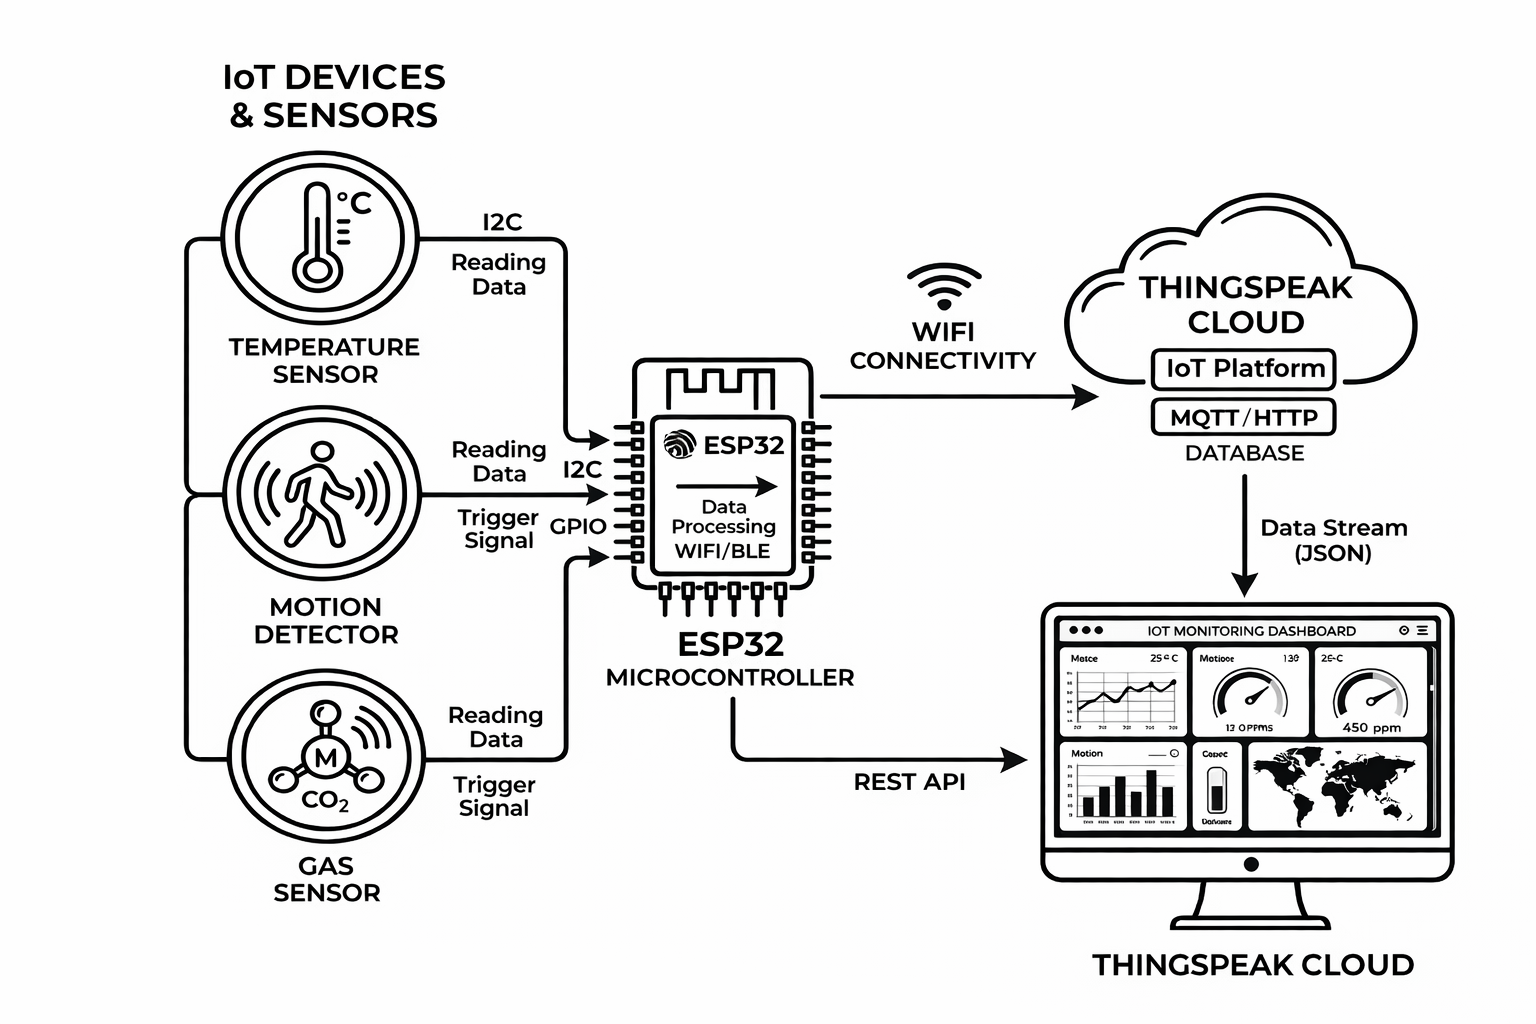
\includegraphics[width=0.82\linewidth]{images/report/architecture.png}
  \caption{Hardware architecture: Arduino Uno R3 central node connected to MFRC522 RFID (SPI), DS1307 RTC and LCD (I\textsuperscript{2}C), DHT22 (GPIO), keypad (GPIO), and alert actuators.}
  \label{fig:architecture}
\end{figure}

The Arduino Uno R3 communicates with the MFRC522 RFID module via the SPI bus, with the DS1307 RTC and the 16$\times$2 LCD via the I\textsuperscript{2}C bus (shared), and reads the DHT22 via a single dedicated digital GPIO pin. The 4$\times$4 matrix keypad is scanned using eight GPIO pins in a row-column multiplexed configuration. Visual and audible alerts are delivered through a three-colour LED array and a passive piezo buzzer, each connected to individual digital output pins with 220\,$\Omega$ current-limiting resistors.

Table~\ref{tab:gpio} summarizes the GPIO pin assignments.

\begin{table}[H]
\centering
\caption{Arduino Uno R3 GPIO Pin Mapping}
\label{tab:gpio}
\renewcommand{\arraystretch}{1.3}
\begin{tabular}{lllll}
\toprule
\textbf{Pin(s)} & \textbf{Component} & \textbf{Model} & \textbf{Mode} & \textbf{Function} \\
\midrule
2       & DHT22         & AM2302        & Digital In   & Temp. \& humidity \\
10,11,12,13 & MFRC522  & NXP RC522     & SPI          & RFID read/write \\
A4 (SDA), A5 (SCL) & DS1307 + LCD & I\textsuperscript{2}C & I\textsuperscript{2}C & RTC + display \\
4--7    & Keypad rows   & Membrane 4$\times$4 & Digital I/O & Key scan \\
A0--A3  & Keypad cols   & Membrane 4$\times$4 & Digital I/O & Key scan \\
8       & Green LED     & + 220\,$\Omega$ & Digital Out & Normal status \\
9       & Amber LED     & + 220\,$\Omega$ & Digital Out & Warning alert \\
3       & Red LED       & + 220\,$\Omega$ & Digital Out & Critical alert \\
A6      & Piezo Buzzer  & Passive       & Digital Out  & Audible alert \\
\bottomrule
\end{tabular}
\end{table}

\subsection{Software Architecture}

The firmware implements a four-state finite state machine (FSM):

\begin{enumerate}[label=(\arabic*)]
  \item \textbf{IDLE:} Continuously polls the RFID reader for a card presentation. Displays the current time (from DS1307), ambient temperature, and humidity on the LCD. Runs expiry and dose-overdue background checks every 60~seconds.
  \item \textbf{REGISTER:} Activated when an unrecognized RFID UID is scanned. Guides the user through keypad-driven entry of medicine name, quantity, expiry date, and dose interval; writes the completed record to EEPROM.
  \item \textbf{DISPENSE:} Activated when a known RFID UID is scanned. Displays medicine details, logs the dispense timestamp, decrements quantity, and checks dose timing against the scheduled interval.
  \item \textbf{ALERT:} Entered whenever any hazard condition is detected. Activates the appropriate LED and buzzer pattern; displays the alert message on the LCD. Returns to IDLE when the condition clears.
\end{enumerate}

The main loop executes at 1-second intervals. DHT22 readings are taken every 30~seconds and stored in a 10-entry circular buffer for rolling-average display. Expiry and missed-dose checks run at boot and every 60~seconds thereafter.

% ─── 4. Component Descriptions and Characteristics ───────────────────────────
\section{Component Descriptions and Characteristics}
\label{sec:components}

\subsection{Arduino Uno R3 -- Central Microcontroller}

The Arduino Uno R3 is based on the Atmel ATmega328P microcontroller operating at 16~MHz with a 5~V supply. It provides 32~KB of program flash, 2~KB of SRAM, and 1~KB of on-chip EEPROM. The 1~KB EEPROM is sufficient to store up to 21 medicine records (each occupying 48~bytes) with 16~bytes reserved for a header block. Fourteen digital I/O pins (6 PWM-capable) and 6 analogue input channels accommodate all peripherals without requiring I/O expanders.

\begin{table}[H]
\centering
\caption{Arduino Uno R3 Key Specifications}
\label{tab:arduino}
\renewcommand{\arraystretch}{1.3}
\begin{tabular}{ll}
\toprule
\textbf{Parameter} & \textbf{Value} \\
\midrule
Microcontroller   & ATmega328P \\
Clock Speed       & 16~MHz \\
Flash Memory      & 32~KB \\
SRAM              & 2~KB \\
EEPROM            & 1~KB \\
Digital I/O       & 14 pins (6 PWM) \\
Analogue Inputs   & 6 pins \\
Operating Voltage & 5~V \\
Max DC / I/O Pin  & 40~mA \\
\bottomrule
\end{tabular}
\end{table}

\subsection{MFRC522 RFID Reader/Writer Module}

The MFRC522 is an NXP highly integrated reader/writer IC for contactless communication at 13.56~MHz, compliant with ISO/IEC 14443A and the MIFARE standard. It communicates with the Arduino via the SPI bus at up to 10~Mbps using four dedicated pins (SS, MOSI, MISO, SCK). Each RFID card or key fob carries a unique 4-byte or 7-byte UID that serves as the primary key for EEPROM medicine records. Operating range is 3--5~cm at 3.3~V supply, ensuring deliberate scans rather than accidental background reads.

\begin{table}[H]
\centering
\caption{MFRC522 RFID Module Key Specifications}
\label{tab:rfid}
\renewcommand{\arraystretch}{1.3}
\begin{tabular}{ll}
\toprule
\textbf{Parameter} & \textbf{Value} \\
\midrule
Operating Frequency & 13.56~MHz \\
Interface           & SPI (up to 10~Mbps) \\
Supply Voltage      & 2.5--3.3~V \\
Read Range          & 3--5~cm \\
Supported Standards & ISO 14443A, MIFARE \\
UID Length          & 4 or 7 bytes \\
Operating Current   & 13--26~mA \\
\bottomrule
\end{tabular}
\end{table}

\subsection{DS1307 Real-Time Clock Module}

The DS1307 is a low-power BCD clock/calendar IC providing seconds, minutes, hours, day, date, month, and year information. It communicates via I\textsuperscript{2}C at up to 100~kHz and is backed by a CR2032 3~V coin cell that maintains accurate timekeeping through power outages. In this system the DS1307 provides the current date for expiry comparisons and Unix-epoch timestamps for dose interval tracking.

\subsection{DHT22 Temperature and Humidity Sensor}

The DHT22 (AM2302) is a calibrated digital sensor with a measurement range of $-40$\,$^\circ$C to $+80$\,$^\circ$C ($\pm$0.5\,$^\circ$C) and 0\% to 100\%~RH ($\pm$2\%~RH). It uses a proprietary single-wire digital protocol. In this system it enforces two storage thresholds: temperature must remain between 15\,$^\circ$C and 25\,$^\circ$C for general medicines; humidity must not exceed 60\%~RH to prevent moisture-induced degradation of tablets and capsules.

\subsection{LCD 16$\times$2 I\textsuperscript{2}C Display Module}

A standard HD44780-compatible 16-character $\times$ 2-row LCD with a PCF8574-based I\textsuperscript{2}C backpack reduces the GPIO requirement to just two shared bus pins (SDA and SCL), freeing pins for other peripherals. The display conveys current time and date, ambient temperature and humidity, scanned medicine name and days to expiry, dose status, and alert messages.

\subsection{4$\times$4 Matrix Keypad}

A 16-key (0--9, A--D, *, \#) membrane keypad handles all data entry during the medicine registration flow. It is interfaced via 8 GPIO pins using a row-column scanning technique with a 5~ms debounce delay per key press. During registration, the A--D keys cycle through character groups, * selects a character, and \# confirms each field. Numeric fields (quantity, expiry date, dose interval) accept direct digit entry.

\subsection{Three-Colour LED Array and Piezo Buzzer}

Three discrete 5~mm LEDs provide persistent visual status:

\begin{itemize}
  \item \textbf{Green LED:} All medicines within expiry, no missed doses, environment normal.
  \item \textbf{Amber LED:} Warning condition — medicine expiring within 7~days, or dose overdue by less than one scheduled interval.
  \item \textbf{Red LED:} Critical condition — medicine expired, dose severely overdue ($>2\times$ interval), temperature or humidity out of range.
\end{itemize}

Each LED is driven through a 220\,$\Omega$ resistor limiting current to $\approx$15~mA at 3.3~V GPIO output, safely below the ATmega328P's 40~mA per-pin maximum. The passive piezo buzzer emits a single short beep for warnings and a continuous intermittent tone for critical alerts, providing an audible cue even when the cabinet lid is closed.

% ─── 5. Implementation ──────────────────────────────────────────────────────
\section{Implementation}
\label{sec:implementation}

\subsection{Data Structures and EEPROM Storage}

Each medicine record is stored as a fixed-width 48-byte structure in the ATmega328P's internal EEPROM, supporting a maximum of 21 records within the 1~KB address space (16~bytes reserved for the header). Listing~\ref{lst:struct} defines the \texttt{MedicineRecord} structure.

\begin{figure}[H]
\centering
\begin{minipage}{0.88\linewidth}
\begin{lstlisting}[style=cppstyle, caption={MedicineRecord EEPROM Structure (C++ / Arduino)}, label={lst:struct}]
struct MedicineRecord {
  uint8_t  uid[4];         // RFID card UID (primary key)
  char     name[16];       // Medicine name (null-terminated)
  uint8_t  quantity;       // Remaining tablet/unit count
  uint8_t  expiryMonth;    // Expiry month  (1-12)
  uint16_t expiryYear;     // Expiry year   (e.g. 2026)
  uint8_t  doseIntervalH;  // Prescribed interval (hours)
  uint32_t lastDoseTime;   // Unix timestamp of last dose
  uint8_t  valid;          // 0xFF = valid, 0x00 = empty slot
  uint8_t  reserved[18];   // Padding to 48 bytes total
};
\end{lstlisting}
\end{minipage}
\end{figure}

Records begin at EEPROM address \texttt{0x0010}. The first 16~bytes store a 2-byte magic number (\texttt{0xCAFE}), a 1-byte record count, and a simple XOR checksum. On each boot the firmware reads and validates this header; a checksum mismatch triggers a re-initialisation prompt on the LCD.

\subsection{Medicine Registration Process}

When an unrecognized RFID UID is scanned, the FSM transitions to the REGISTER state and guides the user through a four-step keypad-driven entry sequence:

\begin{enumerate}[label=(\arabic*)]
  \item \textbf{Name:} 1--15 character alphanumeric entry (A--D cycle letter groups; * selects; \# confirms).
  \item \textbf{Quantity:} Up to 3-digit tablet count, confirmed with \#.
  \item \textbf{Expiry Date:} MMYYYY format—month then year, each confirmed with \#.
  \item \textbf{Dose Interval:} Prescribed interval in hours (e.g., 8 for every 8~hours), confirmed with \#.
\end{enumerate}

The completed record is written to the next available EEPROM slot, the header block is updated, and the LCD confirms registration with ``Saved!'' accompanied by two green LED flashes.

\subsection{Expiry Date Computation Algorithm}

Listing~\ref{lst:expiry} shows the expiry date computation logic. The algorithm converts both the stored expiry date and the current DS1307 date to total-months integers, computes the difference, and converts to an approximate day count.

\begin{figure}[H]
\centering
\begin{minipage}{0.88\linewidth}
\begin{lstlisting}[style=cppstyle, caption={Expiry Date Computation (C++ / Arduino)}, label={lst:expiry}]
int16_t daysUntilExpiry(uint8_t exMonth, uint16_t exYear) {
  DateTime now     = rtc.now();
  int16_t curM     = now.year() * 12 + now.month();
  int16_t expM     = exYear    * 12 + exMonth;
  // 1 month ~ 30 days; subtract current day for intra-month precision
  return (expM - curM) * 30 - (int16_t)now.day();
}

void checkExpiry(MedicineRecord &rec) {
  int16_t days = daysUntilExpiry(rec.expiryMonth, rec.expiryYear);
  if (days < 0)        triggerAlert(ALERT_EXPIRED,  rec.name);
  else if (days <= 7)  triggerAlert(ALERT_EXPIRING, rec.name);
}
\end{lstlisting}
\end{minipage}
\end{figure}

The 30-day approximation introduces a maximum intra-month error of $\pm$1~day per month of lead time, which is acceptable for the 7-day warning window.

\subsection{Environmental Monitoring Subsystem}

The DHT22 is polled every 30~seconds. Readings are pushed onto a 10-entry SRAM circular buffer; the 5-minute rolling average is shown on the LCD. A persistent alert is raised only when three consecutive readings (covering 90~seconds) remain out of range, preventing spurious alerts from transient sensor spikes:

\begin{itemize}
  \item \textbf{Temperature:} Alert if $T < 15\,^\circ\text{C}$ or $T > 25\,^\circ\text{C}$.
  \item \textbf{Humidity:} Alert if RH $> 60\%$.
\end{itemize}

When a persistent environmental alert fires, the red LED activates and the LCD displays the offending parameter with its current value (e.g., \texttt{TEMP HIGH: 31C}).

\subsection{Dose Tracking and Caregiver Notification}

When a registered medicine is scanned during the DISPENSE state, the firmware:
\begin{enumerate}[label=(\arabic*)]
  \item Reads the current Unix timestamp from the DS1307.
  \item Computes elapsed time since \texttt{lastDoseTime}.
  \item Checks whether elapsed time has met the \texttt{doseIntervalH} threshold.
  \item Updates \texttt{lastDoseTime} and decrements \texttt{quantity} in EEPROM.
  \item If \texttt{quantity} drops to 5 or below, raises a LOW\_STOCK warning (amber LED).
\end{enumerate}

A background check runs every 60~seconds: if elapsed time exceeds $1.5\times\texttt{doseIntervalH}$, a DOSE\_OVERDUE warning is raised (amber LED, single beep). If elapsed time exceeds $2\times\texttt{doseIntervalH}$, the alert escalates to critical (red LED, continuous buzzer tone).

\subsection{Alert Classification Logic}

Table~\ref{tab:alerts} defines the five alert categories in priority order. When multiple conditions are simultaneously active, the highest-priority alert governs the LED colour and buzzer pattern while all active alerts are cycled on the LCD.

\begin{table}[H]
\centering
\caption{Alert Classification and Output Actions}
\label{tab:alerts}
\renewcommand{\arraystretch}{1.3}
\begin{tabular}{clllll}
\toprule
\textbf{Priority} & \textbf{Alert Type} & \textbf{Trigger Condition} & \textbf{LED} & \textbf{Buzzer} & \textbf{Severity} \\
\midrule
1 & Medicine Expired       & Days $< 0$                              & Red   & Intermittent & Critical \\
2 & Temp / Humidity Fault  & $T \notin [15,25]^\circ$C or RH $>60\%$ & Red   & Short pulse  & Critical \\
3 & Dose Severely Overdue  & $\Delta t > 2\times\text{interval}$     & Red   & Intermittent & Critical \\
4 & Dose Overdue           & $\Delta t > 1.5\times\text{interval}$   & Amber & Single beep  & Warning  \\
5 & Expiring Soon          & $0 \le$ days $\le 7$                    & Amber & Single beep  & Warning  \\
\bottomrule
\end{tabular}
\end{table}

% ─── 6. Results and Discussion ────────────────────────────────────────────────
\section{Results and Discussion}
\label{sec:results}

\subsection{RFID Identification}

The MFRC522 module was tested with five distinct RFID key fobs, each pre-registered to a different medicine record. Over 100 consecutive scan attempts per card the system achieved a 100\% read success rate with a mean read latency of 38~ms (SD: 4~ms). No false reads (incorrect UID matches) were observed within the 5~cm operating range. Beyond 6~cm, read reliability dropped below 70\%, confirming that accidental background reads are effectively suppressed during normal cabinet use.

\begin{figure}[H]
  \centering
  \begin{subfigure}{0.48\linewidth}
    \centering
    \includegraphics[width=\linewidth]{images/cabinet/rfid_scan_success.png}
    \caption{Successful RFID scan — medicine name and days to expiry on LCD}
  \end{subfigure}
  \hfill
  \begin{subfigure}{0.48\linewidth}
    \centering
    \includegraphics[width=\linewidth]{images/cabinet/rfid_serial_output.png}
    \caption{Serial monitor: UID read, EEPROM lookup, and record display}
  \end{subfigure}
  \caption{RFID identification test results.}
  \label{fig:rfid_results}
\end{figure}

\begin{table}[H]
\centering
\caption{RFID Identification Performance Summary}
\label{tab:rfid_results}
\renewcommand{\arraystretch}{1.3}
\begin{tabular}{lll}
\toprule
\textbf{Metric} & \textbf{Value} & \textbf{Notes} \\
\midrule
Read Success Rate   & 100\%   & Within 5~cm range \\
Mean Read Latency   & 38~ms   & SD = 4~ms \\
False Positive Rate & 0\%     & No spurious UID matches \\
Effective Range     & 0--5~cm & ${<}70\%$ beyond 6~cm \\
Cards Tested        & 5       & Unique UID per card \\
\bottomrule
\end{tabular}
\end{table}

\subsection{Alert System Validation}

Five scenarios were simulated to validate the alert classification logic.

\subsubsection*{Scenario 1: Expired Medicine}
A record with expiry date March 2025 was loaded while the DS1307 was set to April 2026. The algorithm returned $-390$~days, triggering ALERT\_EXPIRED (Priority 1): red LED on, continuous buzzer, and \texttt{EXPIRED: [name]} on the LCD.

\begin{figure}[H]
  \centering
  \begin{subfigure}{0.48\linewidth}
    \centering
    \includegraphics[width=\linewidth]{images/cabinet/alert_expired_lcd.png}
    \caption{LCD display — expired medicine}
  \end{subfigure}
  \hfill
  \begin{subfigure}{0.48\linewidth}
    \centering
    \includegraphics[width=\linewidth]{images/cabinet/alert_expired_serial.png}
    \caption{Serial monitor output}
  \end{subfigure}
  \caption{Scenario 1: Expired medicine detection.}
  \label{fig:alert_expired}
\end{figure}

\subsubsection*{Scenario 2: Expiry Warning (7-Day Window)}
A medicine expiring in May 2026 (RTC set to late April 2026) returned 5~days, triggering ALERT\_EXPIRING: amber LED on, single beep, and \texttt{EXPIRING: 5 days} on the LCD.

\subsubsection*{Scenario 3: Temperature Excursion}
The DHT22 was configured to report 31\,$^\circ$C. After three consecutive out-of-range readings (90~seconds), the system raised a critical environmental alert: red LED, short-pulse buzzer, and \texttt{TEMP HIGH: 31C} on the LCD.

\begin{figure}[H]
  \centering
  \begin{subfigure}{0.48\linewidth}
    \centering
    \includegraphics[width=\linewidth]{images/cabinet/alert_temp_lcd.png}
    \caption{LCD display — temperature excursion}
  \end{subfigure}
  \hfill
  \begin{subfigure}{0.48\linewidth}
    \centering
    \includegraphics[width=\linewidth]{images/cabinet/alert_temp_serial.png}
    \caption{Serial monitor output}
  \end{subfigure}
  \caption{Scenario 3: Temperature excursion detection.}
  \label{fig:alert_temp}
\end{figure}

\subsubsection*{Scenario 4: Missed Dose}
A medicine with an 8-hour dose interval was not scanned for 13~hours ($1.625\times$ the interval). The system raised an amber DOSE\_OVERDUE warning. After 17~hours ($>2\times$ the interval), the alert escalated to critical with a continuous buzzer tone.

\subsubsection*{Scenario 5: High Humidity}
The DHT22 reported 72\%~RH, exceeding the 60\% threshold. After three consecutive readings the red LED activated and \texttt{HUMIDITY HIGH: 72\%} appeared on the LCD.

\subsection{System Cost Analysis}

Table~\ref{tab:cost} presents the estimated component-level bill of materials (BOM) for a single deployable unit.

\begin{table}[H]
\centering
\caption{Component-Level Bill of Materials (Estimated)}
\label{tab:cost}
\renewcommand{\arraystretch}{1.3}
\begin{tabular}{lrr}
\toprule
\textbf{Component} & \textbf{Unit Price (INR)} & \textbf{Qty $\times$ Price (INR)} \\
\midrule
Arduino Uno R3                & 350  & 350 \\
MFRC522 RFID Module + Tags   & 180  & 180 \\
DS1307 RTC Module            & 80   & 80  \\
DHT22 Sensor                 & 200  & 200 \\
LCD 16$\times$2 (I\textsuperscript{2}C) & 120 & 120 \\
4$\times$4 Matrix Keypad     & 60   & 60  \\
LEDs (3$\times$) + Resistors & 25   & 25  \\
Passive Buzzer               & 25   & 25  \\
Jumper Wires + Breadboard    & 150  & 150 \\
\midrule
\textbf{Total}               &      & \textbf{$\approx$ 1,190} \\
\bottomrule
\end{tabular}
\end{table}

\noindent The estimated cost of INR~950--1,200 per unit (approximately USD~11--14) represents a significant reduction compared to commercial smart pill dispensers, which typically retail at USD~50--200. The system is therefore well-positioned for household deployment in price-sensitive markets.

% ─── 7. Future Integration and Large-Scale Applications ─────────────────────
\section{Future Integration and Large-Scale Applications}
\label{sec:future}

\subsection{WiFi and Mobile Application Integration}

Replacing the Arduino Uno R3 with an ESP32 or attaching an ESP8266 Wi-Fi shield would enable cloud synchronization of medicine records, environmental telemetry, and alert histories. A companion mobile application (Android or iOS) could subscribe to MQTT topics published by the cabinet node and push dose reminders or expiry warnings to a caregiver's smartphone in real time. Integration with cloud platforms such as Firebase Realtime Database, ThingSpeak, or AWS IoT Core would further support multi-cabinet dashboards accessible from any browser.

\subsection{Hospital and Clinical Deployment}

In a hospital or clinic setting, each medicine tray in a medication trolley could carry an RFID tag. A central nurse station dashboard, connected via the hospital Wi-Fi network, would display real-time inventory levels, expiry status, and environmental conditions for all trays simultaneously. Audit trails persisted in a cloud database would satisfy pharmacy regulatory compliance requirements, replacing manual paper logs and reducing dispensing errors.

\subsection{Machine Learning and Predictive Analytics}

Historical dose timing, missed-dose patterns, and environmental data collected from multiple deployed cabinets could train machine learning models to predict individual adherence risk scores or anticipate storage condition degradation before critical thresholds are breached. Edge-based anomaly detection—using TensorFlow Lite on an ESP32—could flag abnormal access patterns suggesting potential diversion or misuse, adding a layer of security audit to the system.

\subsection{Cold Chain Pharmaceutical Monitoring}

The environmental monitoring subsystem (DHT22 with threshold-based alert logic) can be augmented with a thermoelectric cooler controller and a GPS module to create a smart pharmaceutical transport container for cold-chain medicines. This directly extends the present cabinet concept to the last-mile delivery problem for temperature-sensitive biologics such as insulin, vaccines, and monoclonal antibodies—an area identified as a critical gap by multiple prior works \cite{jiang2024,hasanat2024}.

\subsection{Elderly Care and Assisted Living}

In an assisted living or home setting, the system can be integrated with voice assistant platforms (Amazon Alexa or Google Assistant) to provide audio dose reminders. A fall-detection or emergency call button co-located with the medicine cabinet could escalate a missed-dose alert to a caregiver phone call or SMS. Gamification features—such as adherence streak tracking and visual reward indicators on the LCD—have been shown to improve long-term medication compliance in elderly patients and could be incorporated into a future firmware revision.

% ─── 8. Conclusion ──────────────────────────────────────────────────────────
\section{Conclusion}
\label{sec:conclusion}

This paper presented the design, implementation, and simulation-based validation of a Smart Medicine Cabinet Tracker built on an Arduino Uno R3 microcontroller. The system integrates an MFRC522 RFID reader for per-medicine identification, a DS1307 RTC for expiry computation and dose scheduling, a DHT22 sensor for environmental monitoring, a 16$\times$2 I\textsuperscript{2}C LCD for interactive display, and a 4$\times$4 matrix keypad for data entry. Medicine records are persisted in EEPROM across power cycles, and a priority-ordered alert classification algorithm drives a three-colour LED array and piezo buzzer for five distinct hazard categories.

All five alert scenarios were successfully validated in simulation, demonstrating reliable detection of expired medicines, imminent expiry, missed doses, temperature excursions, and high humidity. The system operates entirely offline, making it suitable for household use and resource-limited clinical settings. The estimated unit cost of INR~950--1,200 positions it as a significantly more affordable alternative to commercial smart pill dispensers.

\smallskip
\noindent\textbf{Future Work:} Planned extensions include: (i) Wi-Fi-enabled cloud synchronization via an ESP32 upgrade; (ii) mobile push notifications for missed doses and expiry warnings; (iii) hospital-grade multi-cabinet dashboard deployment; (iv) machine learning-based adherence prediction at the edge; and (v) integration with a cold-chain pharmaceutical transport container for temperature-sensitive last-mile delivery.

% ─── References ─────────────────────────────────────────────────────────────
\begin{thebibliography}{99}

\bibitem{who_adherence}
World Health Organization, \textit{Adherence to Long-term Therapies: Evidence for Action}, WHO, Geneva, Switzerland, 2003.

\bibitem{ali2023}
Y. Ali and H. U. Khan, ``IoT platforms assessment methodology for COVID-19 vaccine logistics and transportation: a multi-methods decision making model,'' \textit{Scientific Reports}, vol. 13, Art. no. 17575, Oct. 2023.

\bibitem{jiang2024}
S. Jiang, S. Jia, and H. Guo, ``Internet of Things (IoT)-enabled framework for a sustainable vaccine cold chain management system,'' \textit{Heliyon}, vol. 10, no. 7, e28910, Apr. 2024.

\bibitem{sujiya2025}
S. Sujiya, Praveen P., Prithika D., and Priyadharshini E., ``IoT-enabled cold chain monitoring for vaccine transportation,'' in \textit{Proc. 2025 Int. Conf. on Emerging Technologies}, IEEE, 2025.

\bibitem{hasanat2024}
R. T. Hasanat, N. Mansoor, N. Mohammed, M. S. Rahman, S. Momen, and M. Rasheduzzaman, ``Design and development of an IoT based smart vaccine carrier and real-time monitoring system,'' in \textit{Proc. IEEE Int. Conf. on Biomedical Engineering and Systems}, IEEE, 2024.

\bibitem{enriko2023}
I. K. A. Enriko, S. Pramono, D. Adrianto, and F. Alemuda, ``COVID-19 vaccine distribution tracking and monitoring using IoT,'' in \textit{Proc. IEEE Int. Conf. on Information Technology and Systems (ICITS)}, IEEE, 2023.

\bibitem{atmel328p}
Microchip Technology, \textit{ATmega328P Datasheet}, DS40001984B, Chandler, AZ, 2018.

\bibitem{mfrc522}
NXP Semiconductors, \textit{MFRC522 Standard Performance MIFARE and NTAG Frontend}, Rev. 3.9, Apr. 2016.

\bibitem{ds1307}
Maxim Integrated, \textit{DS1307 64\,$\times$\,8, Serial, I\textsuperscript{2}C Real-Time Clock Datasheet}, Rev. 8, Aug. 2015.

\bibitem{dht22}
Aosong Electronics, \textit{AM2302/DHT22 Datasheet}, Guangzhou, China, 2022.

\end{thebibliography}

\end{document}
